
\begin{enumerate}
    \item We converted these line vectors in augmented matrix form:

\begin{align}
    \myvec{1 & 1 & \vrule & 14\\1 & -1 & \vrule & 4}\\
\end{align} 

Now We will apply Row elementary operation to convert left part of matrix to identity matrix.

\begin{align}
    \xleftrightarrow[]{R_{2}=R_{2}-R_{1}} \myvec{1 & 1 & \vrule & 14\\1 & -2 & \vrule & -10}
\\
    \xleftrightarrow[]{R_{2}=\frac{R_{2}}{-2}} \myvec{1 & 1 & \vrule & 14\\0 & 1 & \vrule & 5}
\\
    \xleftrightarrow[]{R_{1}=R_{1}-R_{2}} \myvec{1 & 0 & \vrule & 9\\0 & 1 & \vrule & 5}
\end{align}

As left part is converted into a identity matrix the intersection vector is \myvec{9 \\ 5}
    

\begin{figure}[!ht]
    \centering
    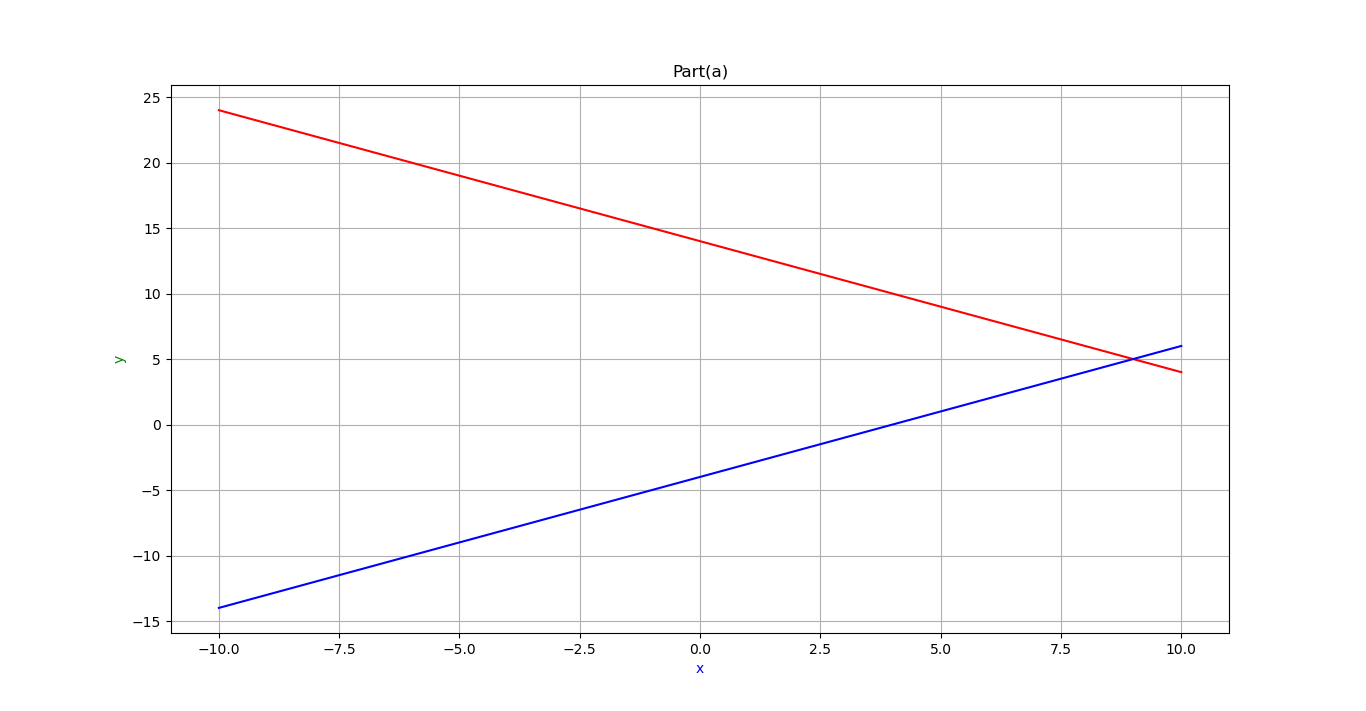
\includegraphics[width=\columnwidth]{./solutions/line_plane/18/figures//A1_parta}
\caption{part(a)}
\label{fig:solutions/line_plane/18/ part(a)}
\end{figure}

\item We converted these line vectors in augmented matrix form: 

\begin{align}
    \myvec{1 & -1 & \vrule & 3\\\cfrac{1}{3} & \cfrac{1}{2} & \vrule & 6}
\\ 
    \xleftrightarrow[]{R_{2}=6\times R_{2}}  \myvec{1 & -1 & \vrule & 3\\2 & 3 & \vrule & 36}
\\ 
    \xleftrightarrow[]{R_{2}=R_{2}-2\times R_{1}} \myvec{1 & -1 & \vrule & 3\\0 & 5 & \vrule & 30}
\\ 
    \xleftrightarrow[]{R_{2}=\frac{R_{2}}{5}} \myvec{1 & -1 & \vrule & 3\\0 & 1 & \vrule & 6}
\\ 
    \xleftrightarrow[]{R_{1}=R_{1}+R_{2}} \myvec{1 & 0 & \vrule & 9\\0 & 1 & \vrule & 6}
\end{align}

As left part is converted into a identity matrix the intersection vector is \myvec{9 \\ 6}


\begin{figure}[!ht]
    \centering
    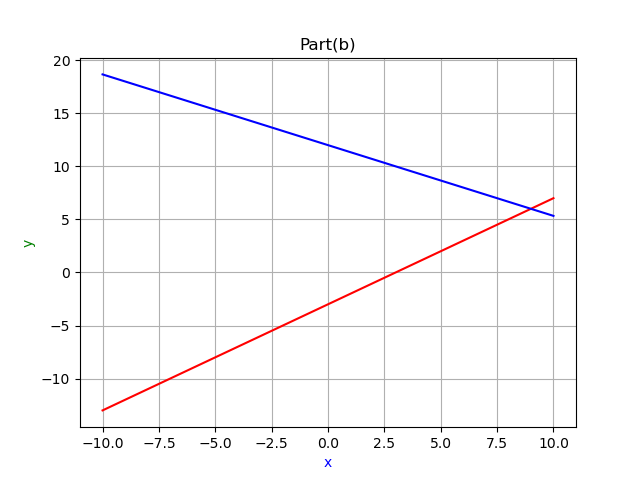
\includegraphics[width=\columnwidth]{./solutions/line_plane/18/figures//A1_partb}
\caption{part(b)}
\label{fig:solutions/line_plane/18/ part(b)}
\end{figure}

\item We converted these line vectors in augmented matrix form: 

\begin{align}
    \myvec{3 & -1 & \vrule & 3\\9 & -3 & \vrule & 9}
\\
    \xleftrightarrow[]{R_{2}=\frac{R_{2}}{3}} \myvec{1 & -1 & \vrule & 3\\1 & -1 & \vrule & 3}
\end{align}

As $R_{1}=R_{2}$ , left part can never be converted into a identity matrix , and we can see now both row are same that means both lines are same they intersect at infinitely many points.


\begin{figure}[!ht]
    \centering
    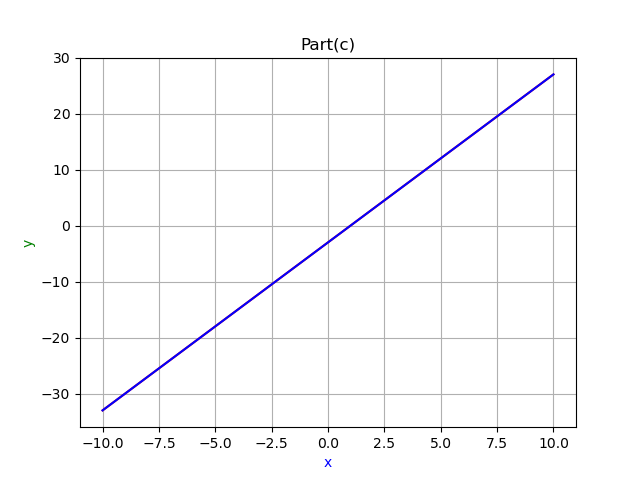
\includegraphics[width=\columnwidth]{./solutions/line_plane/18/figures/A1_partc}
\caption{part(c)}
\label{fig:solutions/line_plane/18/ part(c)}
\end{figure}

\item We converted these line vectors in augmented matrix form: 

\begin{align}
    \myvec{0.2 & 0.3 & \vrule & 1.3\\0.4 & 0.5 & \vrule & 2.3}
\\
    \xleftrightarrow[]{R_{2}=R_{2}-2\times R_{1}} \myvec{0.2 & 0.3 & \vrule & 1.3\\0 & -0.1 & \vrule & -0.3}
\\
    \xleftrightarrow[]{R_{2}=\frac{R_{2}}{-0.1}} \myvec{0.2 & 0.3 & \vrule & 1.3\\0 & 1 & \vrule & 3}
\\
    \xleftrightarrow[]{R_{1}=R_{1}-0.3 \times R_{2}} \myvec{0.2 & 0 & \vrule & 0.4\\0 & 1 & \vrule & 3}
\\
    \xleftrightarrow[]{R_{1}=\frac{R_{1}}{0.2}} \myvec{1 & 0 & \vrule & 2\\0 & 1 & \vrule & 3}
\end{align}

As left part is converted into a identity matrix the intersection vector is \myvec{2 \\ 3}


\begin{figure}[!ht]
    \centering
    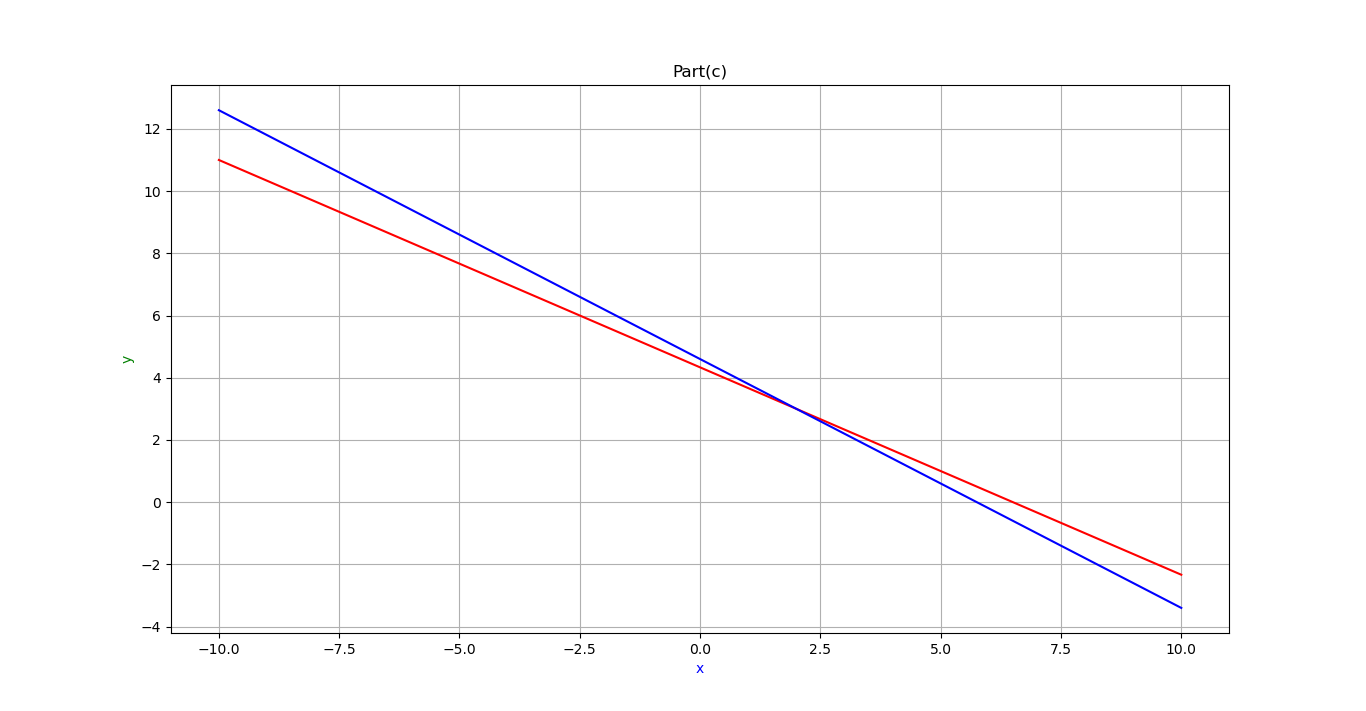
\includegraphics[width=\columnwidth]{./solutions/line_plane/18/figures//A1_partd}
\caption{part(d)}
\label{fig:solutions/line_plane/18/ part(d)}
\end{figure}

\item We converted these line vectors in augmented matrix form:

\begin{align}
    \myvec{\sqrt{2} & \sqrt{3} & \vrule & 0\\\sqrt{3} & \sqrt{8} & \vrule & 0}
\\
    \xleftrightarrow[]{R_{2}=R_{2}-\frac{\sqrt{3}}{\sqrt{2}}\times R_{1}} \myvec{\sqrt{2} & \sqrt{3} & \vrule & 0\\0 & \cfrac{1}{\sqrt{2}} & \vrule & 0}
\end{align}

As we see whatever operation we are applying last column of our augmented matrix remains zero.So the lines are homogeneous lines and they always pass through  origin , the intersection vector is \myvec{0 \\ 0}


\begin{figure}[!ht]
    \centering
    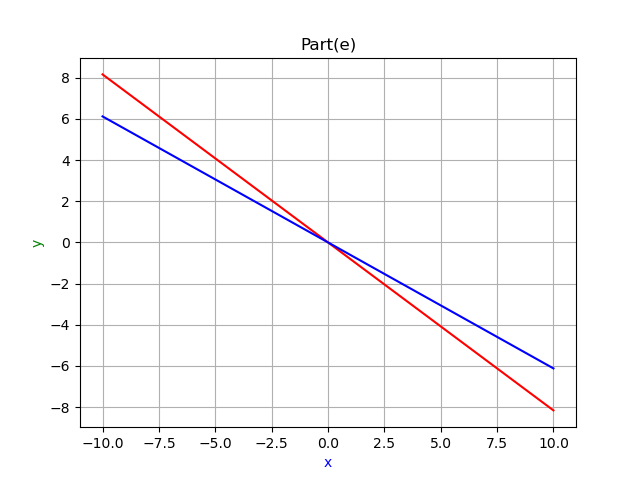
\includegraphics[width=\columnwidth]{./solutions/line_plane/18/figures//A1_parte}
\caption{part(e)}
\label{fig:solutions/line_plane/18/ part(e)}
\end{figure}

\item We converted these line vectors in augmented matrix form: 

\begin{align}
    \myvec{\cfrac{3}{2} & \cfrac{-5}{3} & \vrule & -2\\\cfrac{1}{3} & \cfrac{1}{2} & \vrule & \cfrac{13}{6}}
\\
    \xleftrightarrow[]{R_{1}=6\times R_{1}}
    \xleftrightarrow[]{R_{2}=6\times R_{2}} \myvec{9 & -10 & \vrule & -12\\2 & 3 & \vrule & 13}
\\
    \xleftrightarrow[]{R_{1}=R_{1}-4\times R_{2}} \myvec{1 & -22 & \vrule & -64\\2 & 3 & \vrule & 13}
\\
    \xleftrightarrow[]{R_{2}=R_{2}-2\times R_{1}}  \myvec{1 & -22 & \vrule & -64\\0 & 47 & \vrule & 141}
\\
    \xleftrightarrow[]{R_{2}=\frac{R_{2}}{47}}  \myvec{1 & -22 & \vrule & -64\\0 & 1 & \vrule & 3}
\\
    \xleftrightarrow[]{R_{1}=R_{1}+22\times R_{2}} \myvec{1 & 0 & \vrule & 2\\0 & 1 & \vrule & 3}
\end{align}

As left part is converted into a identity matrix the intersection vector is \myvec{2 \\ 3}


\begin{figure}[!ht]
    \centering
    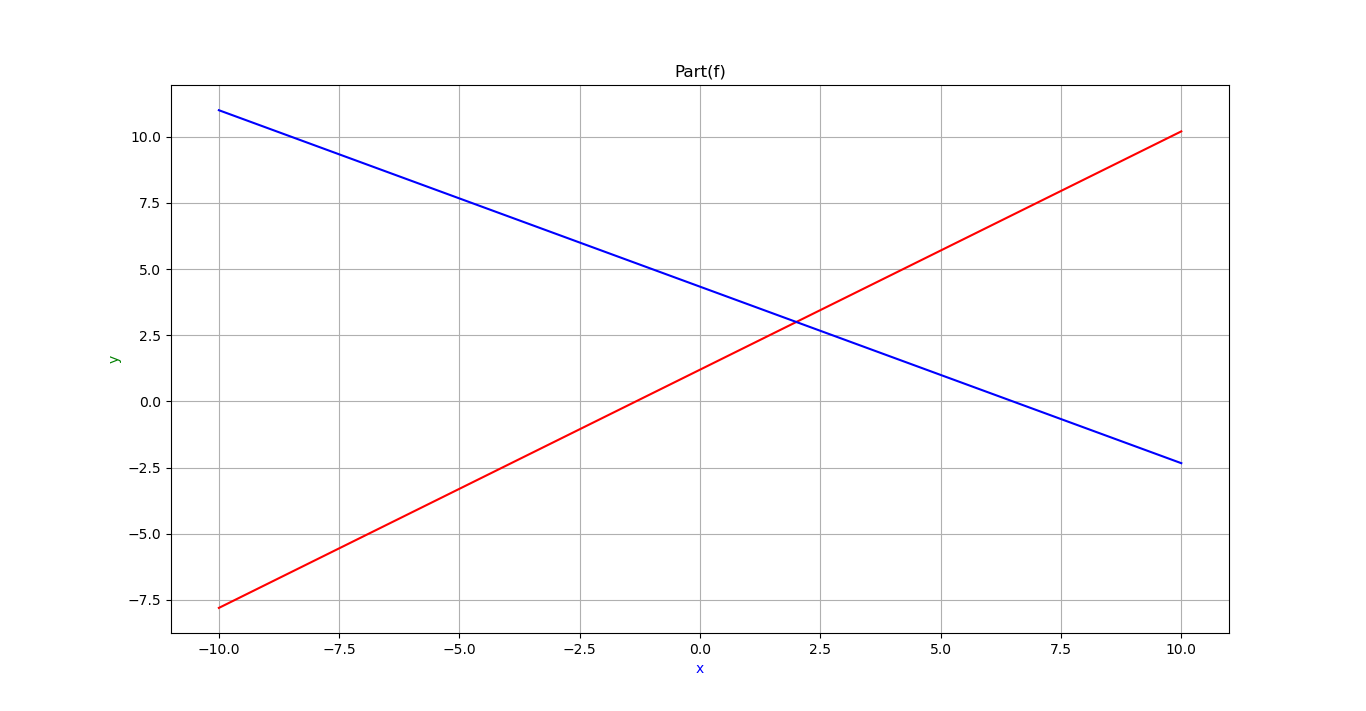
\includegraphics[width=\columnwidth]{./solutions/line_plane/18/figures//A1_partf}
\caption{part(f)}
\label{fig:solutions/line_plane/18/ part(f)}
\end{figure}

\end{enumerate}



